%!TEX root = ../dissertation.tex
\chapter{OpenCog System} \label{cha:opencog_system}

The OpenCog design aims to capture the spirit of the architecture and dynamics of the brain without imitating the details (which are largely unknown) via:
\begin{itemize}
	\item Integrating together a carefully selected combination of cognitive algorithms acting on different kinds of knowledge.
	\item A scalable, robust and flexible C++ software architecture.
	\item A manner specifically designed:
	\begin{itemize}	
	\item To cooperate together with “cognitive synergy” for the scope of tasks characteristic of human intelligence. 
	\item To give rise to the emergence of an effectively functioning knowledge network in the AI system’s mind, as it interacts with the world, including a self-updating hierarchical/heterarchical ontology and models of itself and others.
	\end{itemize}
\end{itemize}
Following section, Section \ref{sec:cognitive_synergy}, elaborates on the new concepts introduced in these points.


\section{Cognitive Synergy}\label{sec:cognitive_synergy}  %% slide 4 tua presentazione, magari aggiungi le parte in basso

OpenCog is a diverse assemblage of cognitive algorithms, each embodying its own innovations. The power of the overall architecture is its careful adherence to the principle of Cognitive Synergy. \\
The human brain consists of a host of subsystems that perform particular tasks, both specialized and general in nature, connected together in a manner enabling them to synergetically assist, rather than work against each other. \\
The essential principles of Cognitive Synergy Theory (CST) can be summarized in the following points, further explored in \cite{inproceedings_cognitive_synergy}:

\begin{enumerate}
	\item Intelligence can be understood as the ability to achieve complex goals in a certain set of environments. 
	\item An intelligent system requires a \enquote{multi-memory} architecture, meaning the possession of a number of specialized yet interconnected knowledge types.
	\item \enquote{Cognitive processes}: a system must possess knowledge creation mechanisms corresponding to each of these memory types.
	\item Each cognitive process must have the ability to recognize when it lacks information and thus, draw it from knowledge creation mechanisms related to other types of knowledge.
	\item The Cognitive Synergy is, therefore, represented by the interaction between the knowledge creation mechanisms, which perform much more effectively in combination than non-interactive mode. 
	\item The activity of the different cognitive processes involved in an intelligent system can be modeled in terms of the schematic implication \enquote{Context \& Procedure $\rightarrow$ Goal}.
\end{enumerate}

These points are implicit in the systems theory of mind given in \cite{goertzel2006the}, where more thorough characterizations of these ideas can be found.\\
Interactions as mentioned in Points 4 and 5 are the conceptual core of CST. \\
Most AI algorithms suffer from combinatorial explosions. In a “general intelligence” context, there is a lack of intrinsic constraint; consequently, the algorithms are unable to filter through all the possibilities (as opposed to a ANI problem like chessplaying, where the context is huge but constrained and hence restricts the scope of possible combinations that needs to be considered). \\
To decrease the severity of combinatorial explosions, one can use an AGI architecture based on CST, in which the different learning mechanisms dealing with a certain sort of knowledge, are designed to synergize with ones dealing with other sorts of knowledge. \\
It is necessary that each learning mechanism recognizes when it is \enquote{blocked} and then, it can ask for help to the other complementary cognitive mechanisms. \\
The Figure \ref{fig:cognitive_processes} is proposed to give a general visual idea of these concepts. It shows an overview of the most important cognitive dynamics considered in Cognitive Synergy Theory and describes the behavior of a system as it pursues a set of goals, which are then refined by inference (through a logic engine or as an emergent process resulting from the dynamics of an Neural Network system), aided by other processes. \\


\begin{figure} [h]
\centering
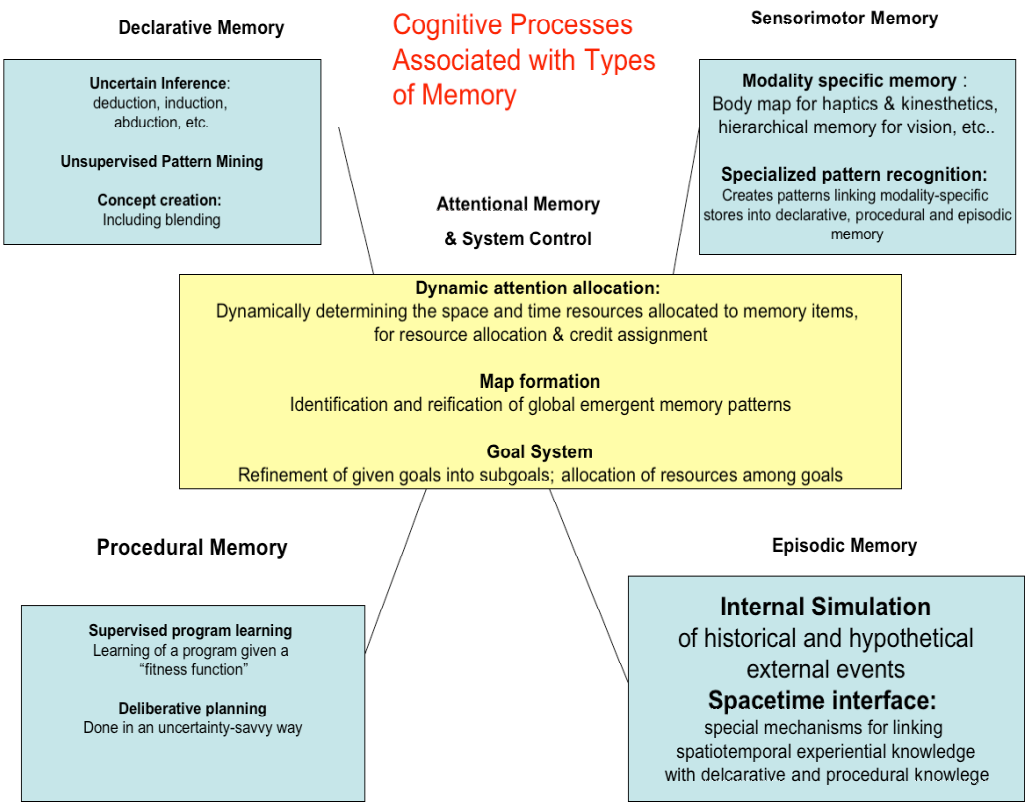
\includegraphics[width=0.7
\textwidth]{figures/Magistrale/04 - cognitive_processes_and_memory}
\caption[Cognitive Processes.]{A high-level overview of the main types of cognitive process considered in Cognitive Synergy Theory, categorized according to the type of knowledge with which each process deals.
\label{fig:cognitive_processes}}
\end{figure} 

The detailed argument explaining how the cognitive algorithm selection and integration methods, chosen by the OpenCog team, will have the desired effect, is sketched on the OpenCog wiki site\footnotemark{} and various previously-published conference papers. It has been presented more thoroughly in the 2014 books Engineering General Intelligence vol. 1 and 2 \cite{DBLP:series/atlantis/GoertzelPG14, DBLP:series/atlantis/GoertzelPG14a}.
\footnotetext{\url{https://wiki.opencog.org/w/Background_Publications}}

\section{OpenCog Architecture}\label{sec:opencog_architecture}

There are several components that make up the basic architecture of OpenCog. In the following sections, they will be described, more or less independently, before being concatenated and contextualized into the problem considered in this project. \\
Currently, the OpenCog project is under strong development and some of the concepts presented here may be obsolete, improved or evolved, or being redesigned. However, much of the basic infrastructure and theory remains unchanged.  

\subsection{Atomspace}\label{sec:atomspace}

The AtomSpace is a platform for building Artificial General Intelligence (AGI) systems. It provides the central knowledge representation component for OpenCog. As such, it is a fairly mature component, on which a lot of other systems are built, and which depend on it for stable, correct operation in a day-to-day production environment. \\
It is a mashup of a large variety of concepts from mathematical logic, theorem proving, graph theory, database theory, type theory, model theory and knowledge representation. \\
More specifically, the OpenCog AtomSpace is an in-RAM knowledge representation database, an associated query engine and graph-re-writing system, and a rule-driven inferencing engine that can apply and manipulate sequences of rules to perform reasoning. \\
The best way to capture all of this, is a kind of in-RAM Generalized Hypergraph (Metagraph) Database. \\
On top of this, the Atomspace provides a variety of advanced features not available anywhere else. It is currently used to store natural language grammars, dictionaries and parsers, to store biochemical and biomedical data, robot control algorithms, machine learning algorithms, audio/video processing pipelines and deep learning neural networks.\\

\subsubsection{Metagraph: a Generalized Hypergraph}\label{sec:gen_hypergraph}

Formally, a graph is:
\begin{itemize}
	\item A set of vertexes $V=\left\{v_{1}, v_{2}, \cdots, v_{M}\right\}$
	\item A set of edges $E=\left\{e_{1}, e_{2}, \cdots, e_{N}\right\}$ where each edge $e_{k}$ is an ordered pair of vertexes drawn from the set $V$.
\end{itemize}
Since edges are ordered pairs, it is conventional to denote them with arrows. In practice, one wishes to associate a label to each vertex, and also some additional attribute data (e.g. weight); likewise for the edges. \\

A hypergraph is very similar to a graph, except for the edges. 
\enquote{Hyperedges} are defined as edges that can contain more than two vertices. That is, the hyperedge, rather than being an ordered pair of vertices, is an ordered list of vertices. \\
Formally, a hypergraph is:
\begin{itemize}
	\item A set of vertexes $V=\left\{v_{1}, v_{2}, \cdots, v_{M}\right\}$
	\item A set of hyperedges $E=\left\{e_{1}, e_{2}, \cdots, e_{N}\right\}$ where each hyperedge $e_{k}$ is an ordered list of vertexes drawn from the set $V$. This list may be empty, or have one, or two, or more members.
\end{itemize}

A good representation of a hypergraph is the one proposed in Figure \ref{fig:atomspace_table}. 
It was a straight-forward extension of the edge table, to which a new column was added for each position and then, those columns were mashed together into one set.  

\begin{figure} [h]
\centering
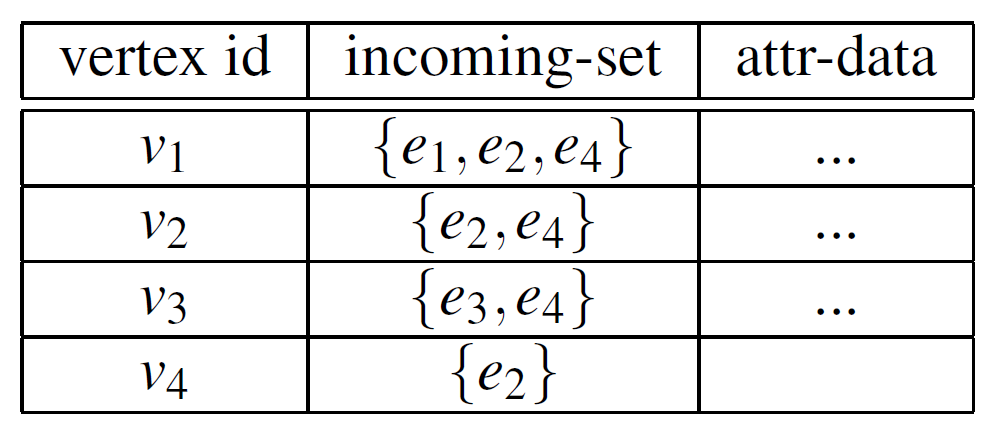
\includegraphics[width=0.7
\textwidth]{figures/Magistrale/atomspace_table}
\caption[Hypergraph edge table]{Hypergraph edge table
\label{fig:atomspace_table}}
\end{figure}

The vertex table looks like the edge table, but the vertex-list is an ordered list, while the incoming-set (the edge-set) really is a set. This is because a hypergraph is “almost” a bipartite graph, having the form of Figure \ref{fig:hypergraph_graph}, with the set E on the left being the set of hyperedges. \\

\begin{figure} [h]
\centering
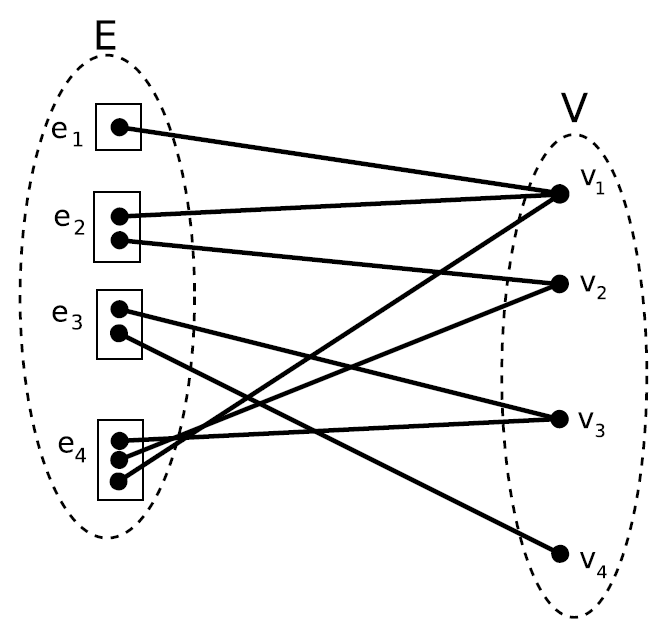
\includegraphics[width=0.6
\textwidth]{figures/Magistrale/hypergraph_graph}
\caption[Hypergraph as bipartite graph]{The $E$ and $V$ ellipses are the hyperedge and vertex tables. The boxes mean that the hyperedges are ordered lists.
\label{fig:hypergraph_graph}}
\end{figure}

Before define a Metagraph, a change of terminology is useful: the basic objects are now called \enquote{Nodes} and \enquote{Links} instead of \enquote{vertexes} and \enquote{edges}. \\
Thus, a Metagraph is:
\begin{itemize}
	\item A set of nodes $V=\left\{v_{1}, v_{2}, \cdots, v_{M}\right\}$
	\item A set of links $E=\left\{e_{1}, e_{2}, \cdots, e_{N}\right\}$ where each hyperedge $e_{k}$ is an ordered list of nodes, or other links, or a mixture. They are arranged to be acyclic (to form a directed acyclic graph).
\end{itemize}

The metagraph is a generalization of a hypergraph, in the sense that now a hyperedge (link) may contain either another vertex (node) or another link. Visually, it has the shape of a Directed Acyclic Graph (DAG), such as the one shown in Figure \ref{fig:metagraph_graph}.

\begin{figure} [h]
\centering
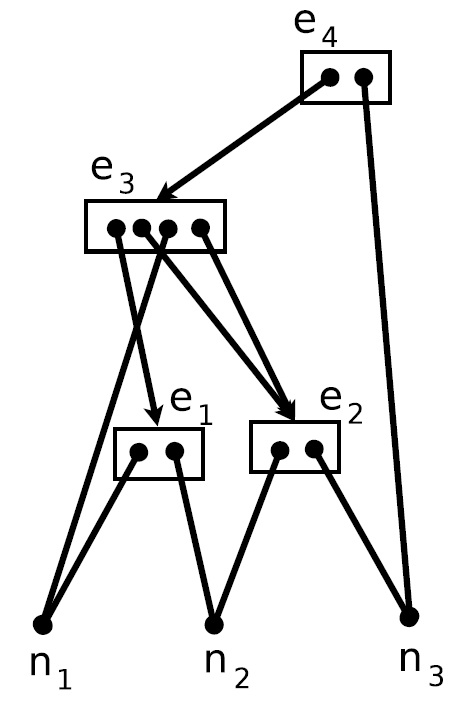
\includegraphics[width=0.4
\textwidth]{figures/Magistrale/metagraph_graph}
\caption[Directed Acyclic Graph ]{An example of a DAG.
\label{fig:metagraph_graph}}
\end{figure}

But in Metagraph, links are ordered lists, represented as boxes. Thus, to convert it in a DAG it is possible to collapse the boxes to single points or to dissolve the boxes entirely and replace a single arrow, from point-to-box, by many arrows, from point to each of the box elements.  \\
Whereas the node table is the same as the vertex table for the hypergraph, nevertheless the link table now requires both an outgoing-atom list and an incoming-link set.
Figure \ref{fig:metagraph_table} shows the result.

\begin{figure} [h]
\centering
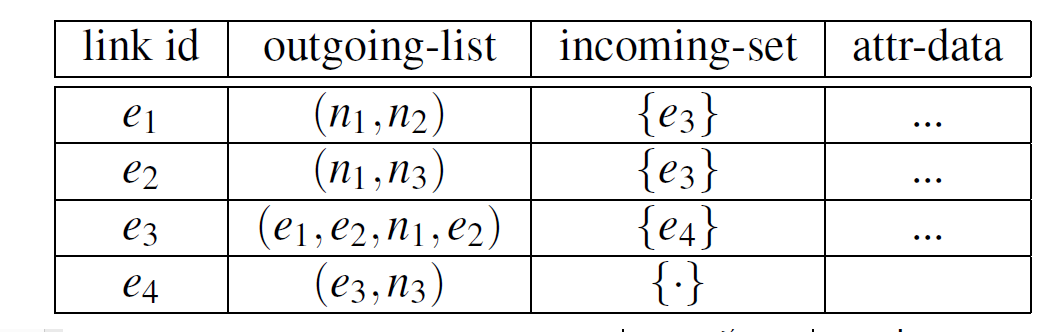
\includegraphics[width=0.8
\textwidth]{figures/Magistrale/metagraph_table}
\caption[Metagraph link table]{Metagraph link table
\label{fig:metagraph_table}}
\end{figure}

For convenience, the name \enquote{Atom} is given to something that is either a node or a link. Links are then, sets of atoms. \\
These concepts are described in \cite{Vep20a, metagraph_app}, where RAM-usage considerations, reasons why metagraphs offer more efficient, more flexible and more powerful ways of representing graphs and reasons why a metagraph store is better than a graph store and much more, can also be found. \\

Finally, some extensions of the metagraph are considered: Typed Metagraph (TMG) and Directed Typed Metagraph (DTMG). \\
Typed metagraphs are defined as hypergraphs with types assigned to hyperedges and their targets, and the potential to have targets of hyperedges connect to whole links, as well as targets. 
An example can be found in Figure \ref{fig:typed_edge}. \\

\begin{figure}[h]
\centering
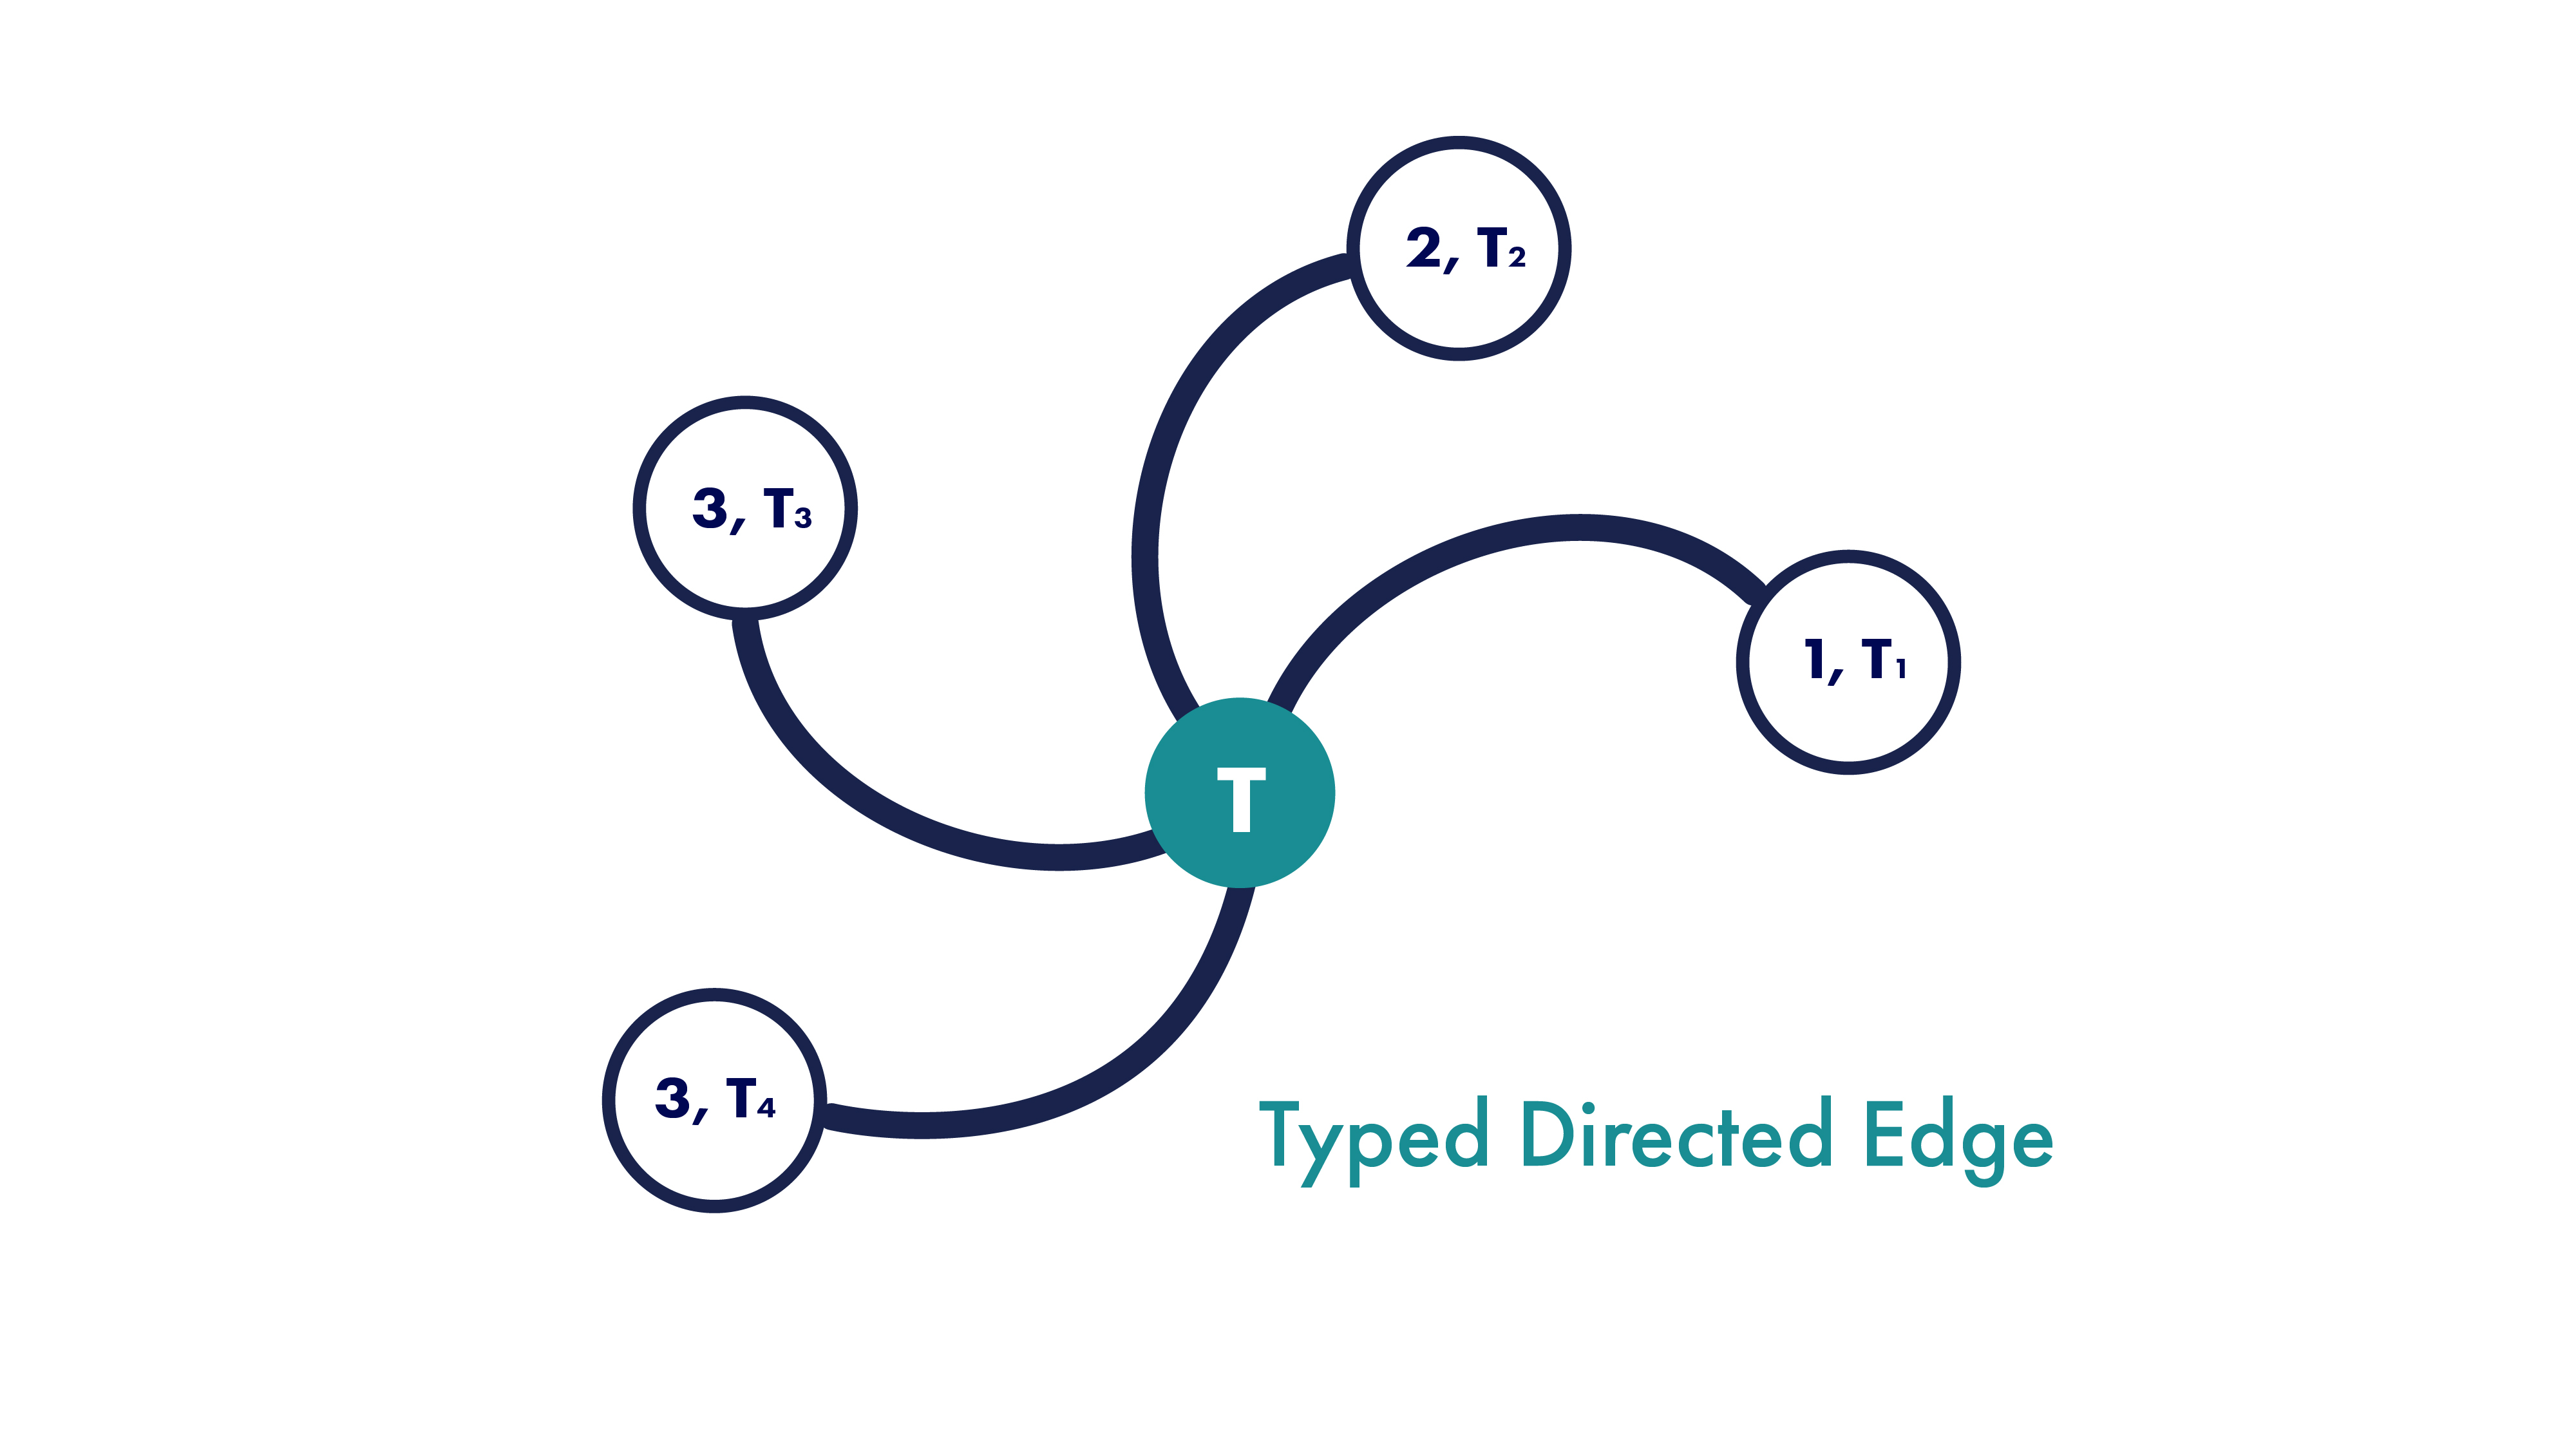
\includegraphics[width=0.6
\textwidth]{figures/Magistrale/typed_edge}
\caption[Typed Directed Edge]{Example of a typed, directed edge. This one has 4 targets. $T$ is the type of the edge itself. The third and fourth targets are unordered relative to each other.
\label{fig:typed_edge}}
\end{figure}

A natural extension of a TMG is the Probabilistically TMG, based on probabilistic dependent types. Thus, one can assign a probability (or an entire probability distribution) to each connection between edges, thanks to the probabilistic type inheritance relations. In this way, it is possible to obtain a KB that can work with probabilistic logic, fuzzy logic, make uncertain inferences and much more. \\
Atomic Directed Typed Metagraphs (atomic DTMG) are introduced via partitioning the targets of each edge in a typed metagraph into input, output and lateral sets; one can then look at \enquote{metapaths} in which edges' output-sets are linked to other edges' input-sets (Figure \ref{fig:typed_metapath}). Thus, a DTMG is generally defined as a TMG composed by connecting DTMGs via metapaths, a recursive definition that bottoms out on the definition of atomic DTMGs. \\
For the whole theoretical formalism concerning TMG and DTMG refer to \cite{DBLP:journals/corr/abs-2012-01759}. 
That paper concludes by also describing useful types of morphisms that can be defined on a DTMG (catamorphisms, anamorphisms, histomorphisms, futumorphisms, hylomorphisms, chrono\-morphisms, metamorphisms and metachronomorphisms). 
They allow to formulate a wide variety of operations on metagraphs, which will not be described here. \\
The important thing to keep in mind is that the KB is used for AGI, so there will be many metagraphs and very large ones. Morphisms allow you to obtain simple and complex results by mutating/transforming/stretching/compressing the metagraph quickly and cleanly. \\
Lastly, it is also useful to associate metagraph edges $E_{i}$ with nite lists $V_{i}$ of Values, each of which may be integer, floating-point or more complex in structure. The reason for these Values will be mentioned later.

\begin{figure}[h]
\centering
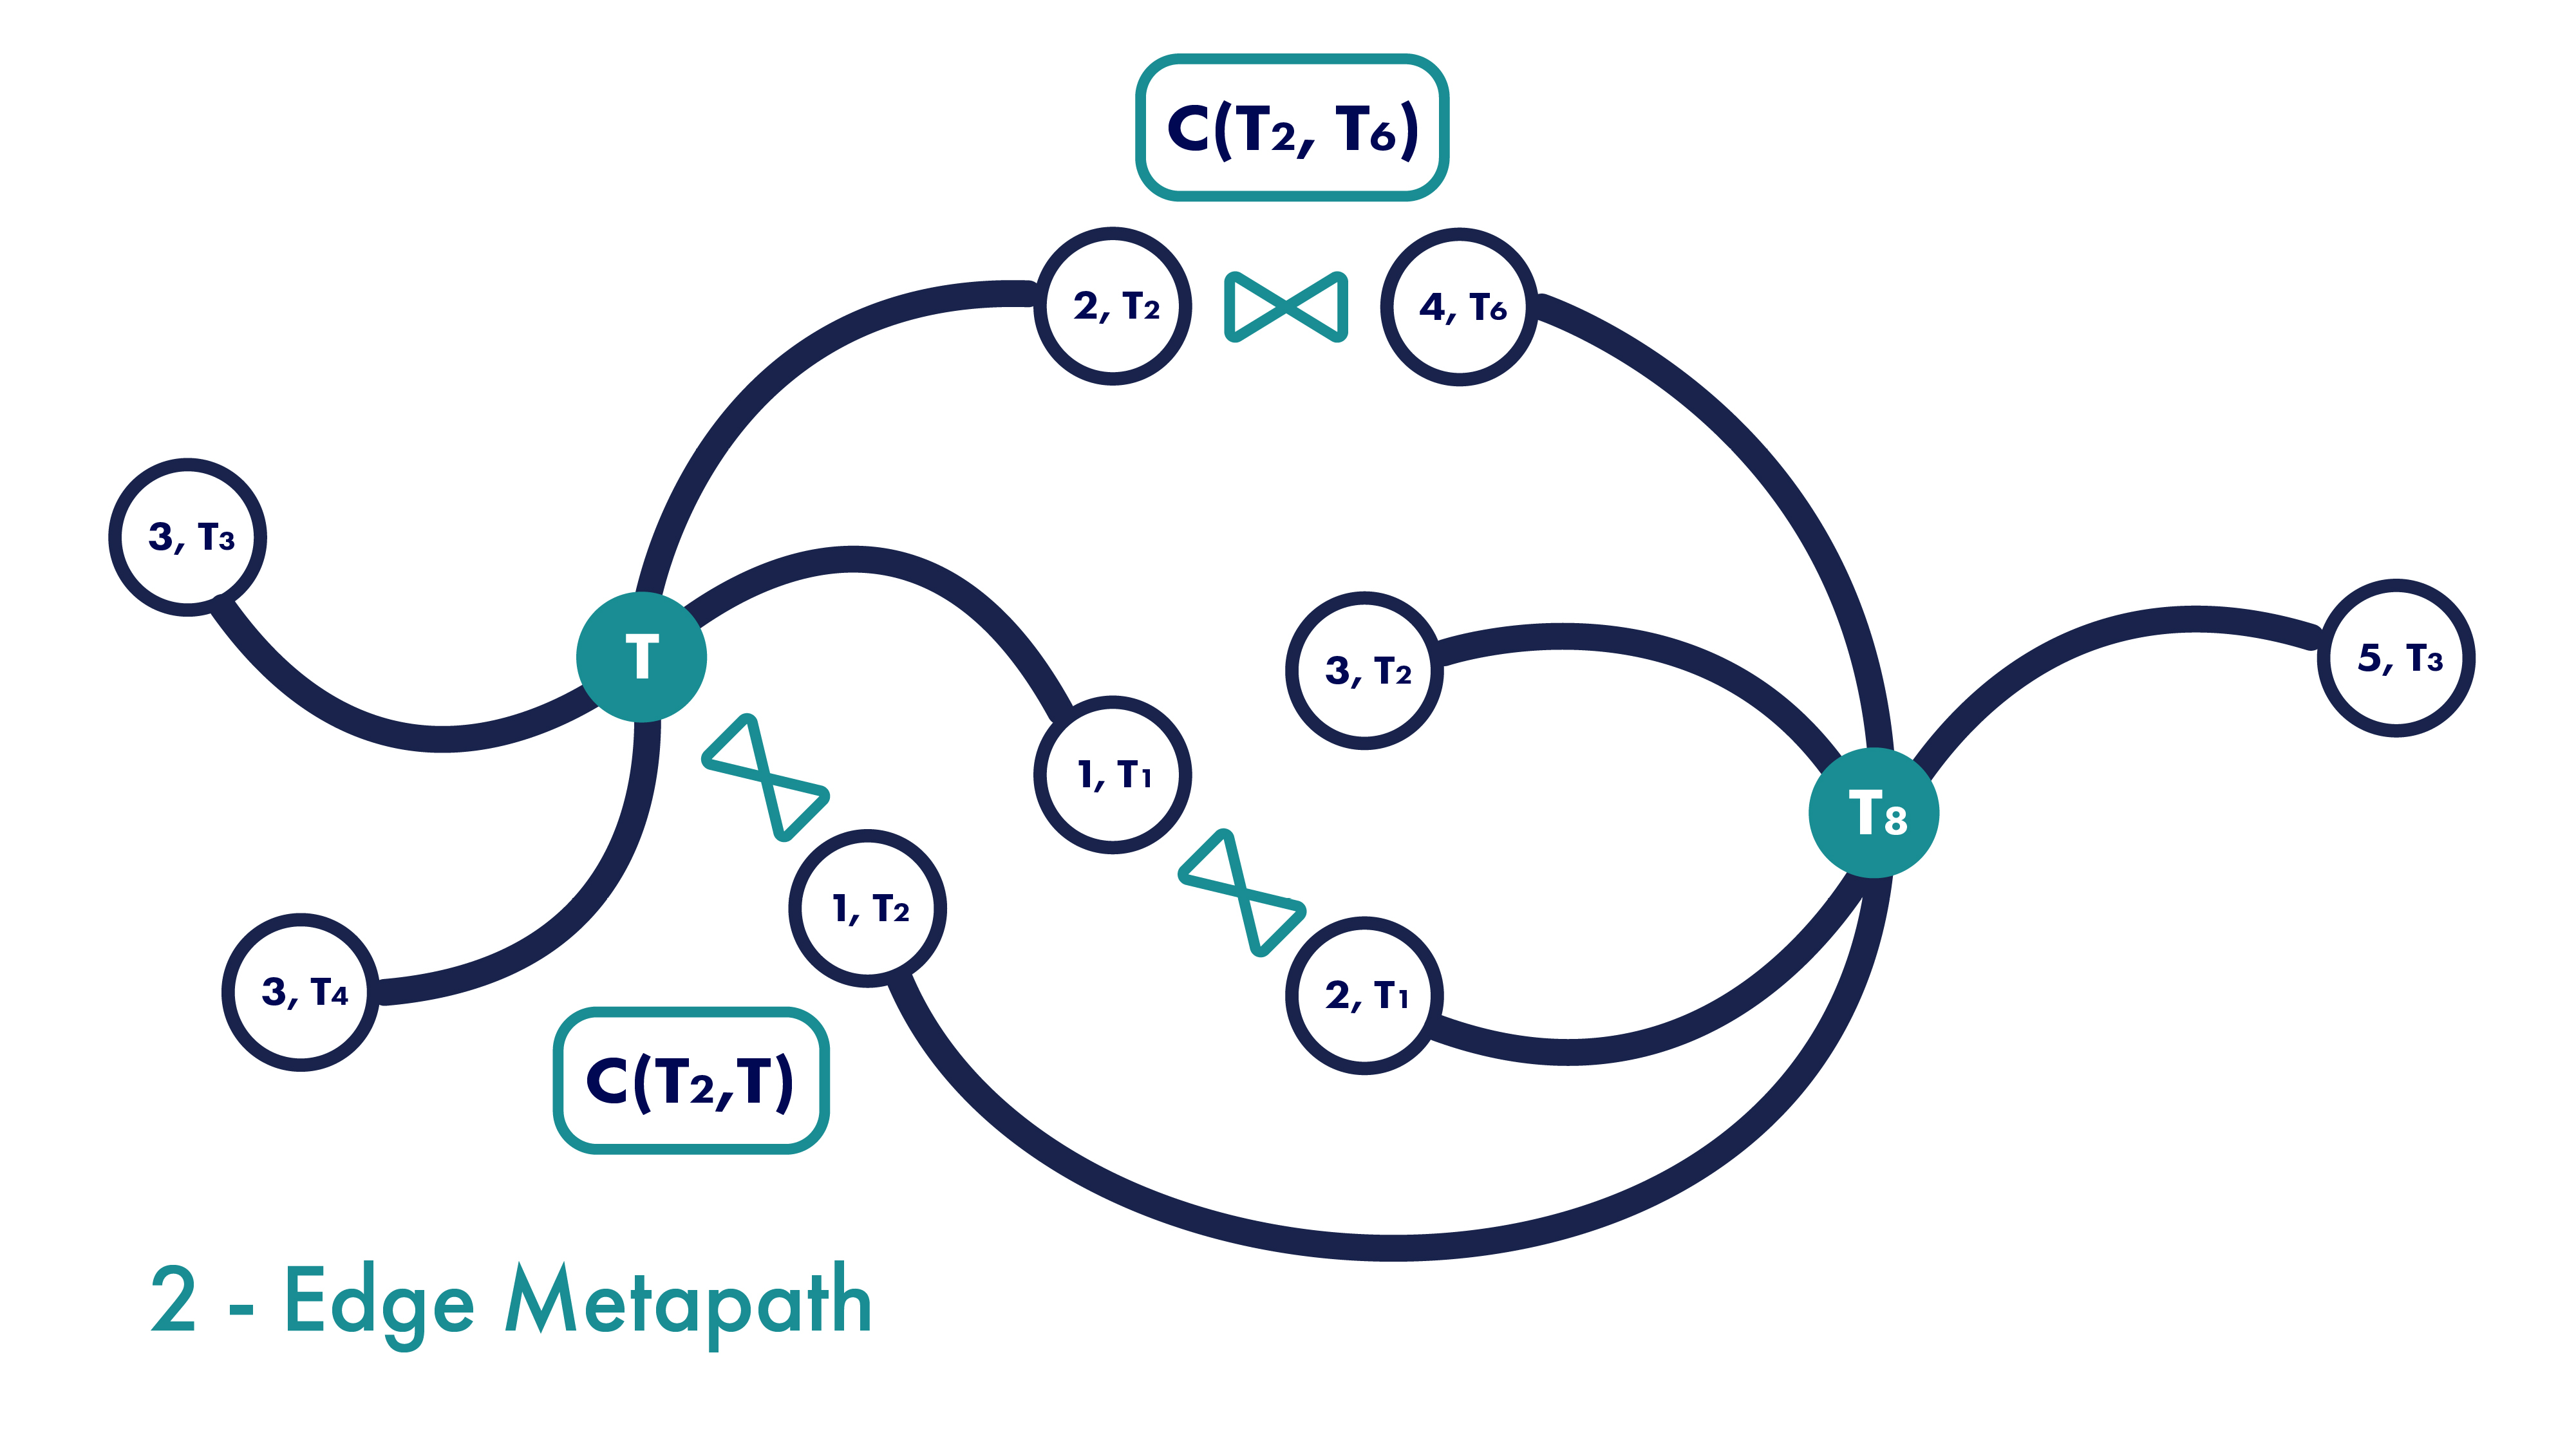
\includegraphics[width=0.65
\textwidth]{figures/Magistrale/typed_metapath}
\caption[Metapath]{A short metapath, formed by connecting two directed edges.
\label{fig:typed_metapath}}
\end{figure}

\subsubsection{Atoms}\label{sec:atoms}

The vertices (nodes) and edges (links) of a graph (metagraph), known as Atoms, are used to represent not only \enquote{data}, but also \enquote{procedures} and then, many metagraphs are executable programs as well as data structures. \\
Atoms are one of the main components of the AtomSpace. Atoms, together with Values are what the AtomSpace stores.  \\
The two primary types of Atoms are Nodes and Links. They are used to represent anything that resembles a graph-theoretical graph. \\
From the TMG definition above, Atoms are typed (in the sense of Type Theory) and thus, they can be used to store a large variety of information. 
Values are used to assign \enquote{valuations} to Atoms, to indicate the truth or likelihood of that Atom, or to hold other kinds of transient data. Every Atom has a key-value database attached to it, that can store any kind of information about that Atom. The distinction between the \enquote{shape of the graph}, and its related \enquote{data} is central for allowing high-speed graph traversal and generalized graph query. Note that, the name \enquote{Atom} was chosen because of the resemblance of OpenCog Atoms to the concept of atoms in mathematical logic. Moreover, in Ruby and Prolog programming languages, symbols are literally called atoms; in both LISP and Guile, allow parameters to be attached to symbols, as Values can be attached to Atoms. \\

When an atom are placed in the AtomSpace, it becomes unique: it gets a single, unique ID. Thus, in comparison to other programming languages\footnotemark{}, Atoms can be understood to be the same thing as symbols. The AtomSpace is essentially a symbol table, which commonly has the unique-symbols property. \footnotetext{Section \ref{sec:atomese} explains why it is possible to talk about programming languages}\\
The atom ID is the string name of a Node and the outgoing set of a Link. Specifically: Nodes are identified by their names or labels, that is the only property that they have. Links are identified by their contents, which are ordered or unordered sets of other atoms. Links do not have any name or label other than their contents: a link is uniquely identified by it's type and it's contents.\\
A TruthValue (a certain type of Values) gives each Atom a valuation or an interpretation and conseguently, all Atoms in a given, fixed AtomSpace always carry a default valuation/interpretation (i.e. a SimpleTruthValue) along with them. Naturally, an Atom may have one or more different kinds of TruthValues. \\
All TruthValues (tv) expose at least two parameters, representative of the SimpleTruthValue (stv):

\begin{enumerate}
	\item Strength: it represents a probability estimate of the true unknown probability. It is a floating-point value ranging from 0 to 1, with 0 denoting the classical Boolean false, and 1.0 denoting true.
	\item Confidence: it captures the spread of the second order distribution over the true unknown probability. It is a floating point value ranging from 0 to 1, expressing the certainty of the strength, with 0 denoting completely uncertain, and 1 denoting completely confident.
\end{enumerate}

The types form a type hierarchy: all atoms inherit from the type \enquote{Atom}, and the type Atom itself inherits from ProtoAtom. The ProtoAtom is itself the base type for Values as well as Atoms.
The atom type category site\footnotemark{} lists all documented theorized, proposed, currently in use, deprecated and obsolete atoms. \\
It is not a complete list: new types are easily invented, and the various OpenCog books mention Atom types that are not implemented or have been implemented in a different way. This reflects a more general point: the specific collection of Atom types in an OpenCog system is bound to change as the system is developed and experimented with. In the current system, it does not necessarily have a profound and lasting significance. \footnotetext{\url{https://wiki.opencog.org/w/Category:Atom_Types}}\\

Following a descriptive list of the main types of atoms used for this project:

\begin{itemize}
	\item \textbf{ConceptNode}: a Node representing any concept. \\
Its TruthValue, composed of at least a strength and a confidence value, has the strength that indicates the occurence of a concept within the context of experience and the confidence that indicates how sure the agent or system is of this value. 
\\
For example, imagine an empty AtomSpace and a newborn agent that begins observing the world for the first time. If the first two things it sees are a man and a cat, it may define the following concepts:

\begin{footnotesize}\textbf{Code in Scheme Programming Language notation:} \\
ConceptNode example.\end{footnotesize}
\begin{python}
	ConceptNode "man" (stv 0.5 0.001)
	ConceptNode "cat" (stv 0.5 0.001)
\end{python}

Since the agent has only observed two concepts in its universe, it will split in two the universe (and Strength accordingly): half (0.5) consists of men and the other half (0.5) consists of cats.
Because the agent has not made a lot of observations yet, it may assign a low Confidence to these values.

	\item \textbf{InheritanceLink}: a Link specify is-a relationships. \\
In the OpenCog system, basic InheritanceLinks are used to specify both intensional (is-a) and extensional (is-an-instance-of) relationships.

\begin{footnotesize}\textbf{Code in Scheme notation:} \\
InheritanceLink example, which specifies that a cat is an animal.
\end{footnotesize}
\begin{python}
	InheritanceLink
		ConceptNode "cat"
		ConceptNode "animal"
\end{python}

In this case, the TruthValue associated to InheritanceLink should be 0, if it is considered as extensional inheritance (inheritance between sets based on their members) and a value greater than 0 in the case of intensional inheritance (inheritance between entity-types based on their properties); obviously the value depends on how the agent assigns it.

	\item \textbf{PredicateNode}: it names the predicate of a relation. \\
Predicates are functions that have arguments, and produce a truth value as output. Predicates in OpenCog roughly resemble the predicate of first-order logic, but more general. It is very similar to a characteristic function in probability theory, which helps assign a floating-point truth value to a declaration. Its usege will be understood at later points. \\
Two interesting type of Atom that are derived from PredicateNode are \textbf{DefinedPredicateNode} and \textbf{GroundedPredicateNode}. \\
The first is a single atom that is attached to a more complex definition. During the evaluation of the predicate, its definition (typically some formula or other complex expression, constituted entirely of Atoms) is looked up and is used during evaluation. \\
The second specifies a predicate whose truth value is updated by the evaluation of a scheme, python or C++ code snippet. It is a \enquote{black box} from the point of view of logical inference and knowledge representation and it is used to interface to external data systems, for example, to robot motor control systems, or to sensory input systems. It is impossible to reason with it, as opposed to DefinedPredicateNodes, which are \enquote{clear boxes} whose inner workings are visible to inference, learning and analysis algorithms.

	\item \textbf{ListLink}: a Link used for grouping Atoms for some purpose, typically to specify a set of arguments to some function or relation. \\
The ListLink is best understood as a Cartesian product\footnotemark{}, because all of its uses involve passing an ordered sequence of arguments to some function or predicate. Ordered sequences can be naturally understood as Cartesian products, which is extremely general, cutting across all branches of mathematics.
\footnotetext{\url{https://github.com/opencog/atomspace/issues/1490\#issuecomment-352961503}}

	\item \textbf{EvaluationLink}: it provides a way for specifying the truth value of a predicate on a set of arguments. \\
The EvaluationLink is the most central and important atom type in OpenCog, as it is how OpenCog implements knowledge representation.

\begin{footnotesize}\textbf{Code in Scheme notation:} \\
EvaluationLink general structure, followed by a pratical example.
\end{footnotesize}
\begin{python}
	EvaluationLink <tv>
   		PredicateNode some_p
   		ListLink
       			SomeAtom val_1
       			OtherAtom val_2
\end{python}
This indicates that the predicate $some\_p$, applied to arguments $val\_1$ and $val\_2$, has the TruthValue $tv = some\_p(val\_1, val\_2)$. \\
Pratical example, $3 < 42$ is true:
\begin{python}
	 EvaluationLink <true_tv>
		PredicateNode "LessThan"
		ListLink
			NumberNode 3
			NumberNode 42
\end{python}

	\item \textbf{QueryLink}: it is used to specify a search pattern that can be grounded, solved or satisfied. Patterns consist of a set of clauses, with each clause containing one or more variables. When executed, the pattern matcher attempts to find groundings for the variables; that is, it attempts to find values for the variables such that the resulting graph exists in the AtomSpace. \\
QueryLink performs graph rewriting: after finding a match for a pattern, it uses the results to create a new pattern. \\
The QueryLink is a 2-ary or a 3-ary link, containing an optional variable declaration, followed by a pattern, followed by an implicand (consequent). In this project is used in a 3-ary form and thus, only the explicitly-declared variables are bounded. \\
QueryLink is treated as a graph re-write rule by the pattern matcher. That is, if the graph P (the antecedent) is found, then the graph Q (the consequent or implicand) is instantiated in the AtomSpace. If the graph Q is an \textbf{ExecutionOutputLink} atom type, such as in this project, then the specified Scheme/Python/C++/etc. routine is executed, with the rest of the ExecutionOutputLink contents passed as arguments. Conceptually, the pattern matcher acts to apply rules, specified as QueryLinks, to the contents of the AtomSpace. It implements a single step of a forward chainer.

\begin{footnotesize}\textbf{Code in Scheme notation:} \\
EvaluationLink general structure, followed by a pratical example.
\end{footnotesize}
\begin{python}
	QueryLink
		$variable_declarations	# optional
		P
		ExecutionOutputLink  	# graph Q
			GroundedSchemaNode "some-routine"
			ListLink
				A_1
				A_2
				...
\end{python}

The expression or predicate P is the pattern to be matched. The variables appearing in P are listed in the \$variable\_declarations. If a match to P is found, the variables are grounded with their matching atoms. The various A\_1, A\_2, etc. are created for each match, and are then passed as the first, second, ... arguments to a function \enquote{some-routine}. This function can then perform any action, for example drives external systems, such as motor controls or other devices.
\end{itemize}

There are other atom types used here. A more general list of Opencog atom types, which can be divided into categories, is the following:

\begin{itemize}
\item Arithmetic Atom Types: EqualLink, GreaterThanLink, NumberNode, IntervalLink, etc.
\item Boolean Atom Types: AndLink, OrLink, NotLink, etc. 
\item All atom types used for Natural Language Processing (NLP)
\item Atom types for the OpenCog Probabilist Logic Network
\item Atom types to perform Pattern Matching (PresentLink, AbsentLink, VariableList / VariableSet / VariableNode, etc.) 
\item Atom types for the threading 
\item Set-theoretical Atom Types: types having some form of set-theoretical signficance (MemberLink, SetLink, SubsetLink, etc.)
\item Atom types to perform searches over the AtomSpace (JoinLink, QueryLink, MeetLink, etc.) 
\end{itemize}

There is a type system for working with atom types: that is, the type of an atom can itself be specified using other atoms, which also applies to the polymorphic types. The type system allows for basic error checking, such as with the type checker, and more generally, it allows type-logical reasoning and inference to be performed on atom signatures. \\

In conclusion, the AtomSpace Explorer web tool can be used to display OpenCog data on screen. Atomese is fetched from the AtomSpace, then displayed as a two dimensional graph in the browser, Figure \ref{fig:atomspace_explorer} provides an example. \\

As closing note of this section, to greatly simplify the work in this project, uncertainty-free inference is used, so all TruthValues associated with atoms are always TRUE, that is what the robot \enquote{sees, does and thinks} has no probability of \enquote{failure}. But, as amply demonstrated above, the system is set up to work in completely uncertain environments and with uncertain reasoning. \\
Indeed, one of the most interesting modules of OpenCog is Probabilistic Logic Networks (PLN), a conceptual, mathematical and computational approach to uncertain inference. Although this project does not use it, it is particularly suitable for uncertain reasoning, especially when knowledge is based on limited observations of reality, but it can also handle abstract mathematical reasoning, and the relationship between the two, therefore this project could be integrated into it in the future. \\
PLN is currently used as a basic module for reasoning algorithms \cite{goertzel2008probabilistic, Goertzel2011RealWorldRT}. 

\begin{figure}[h]
\centering
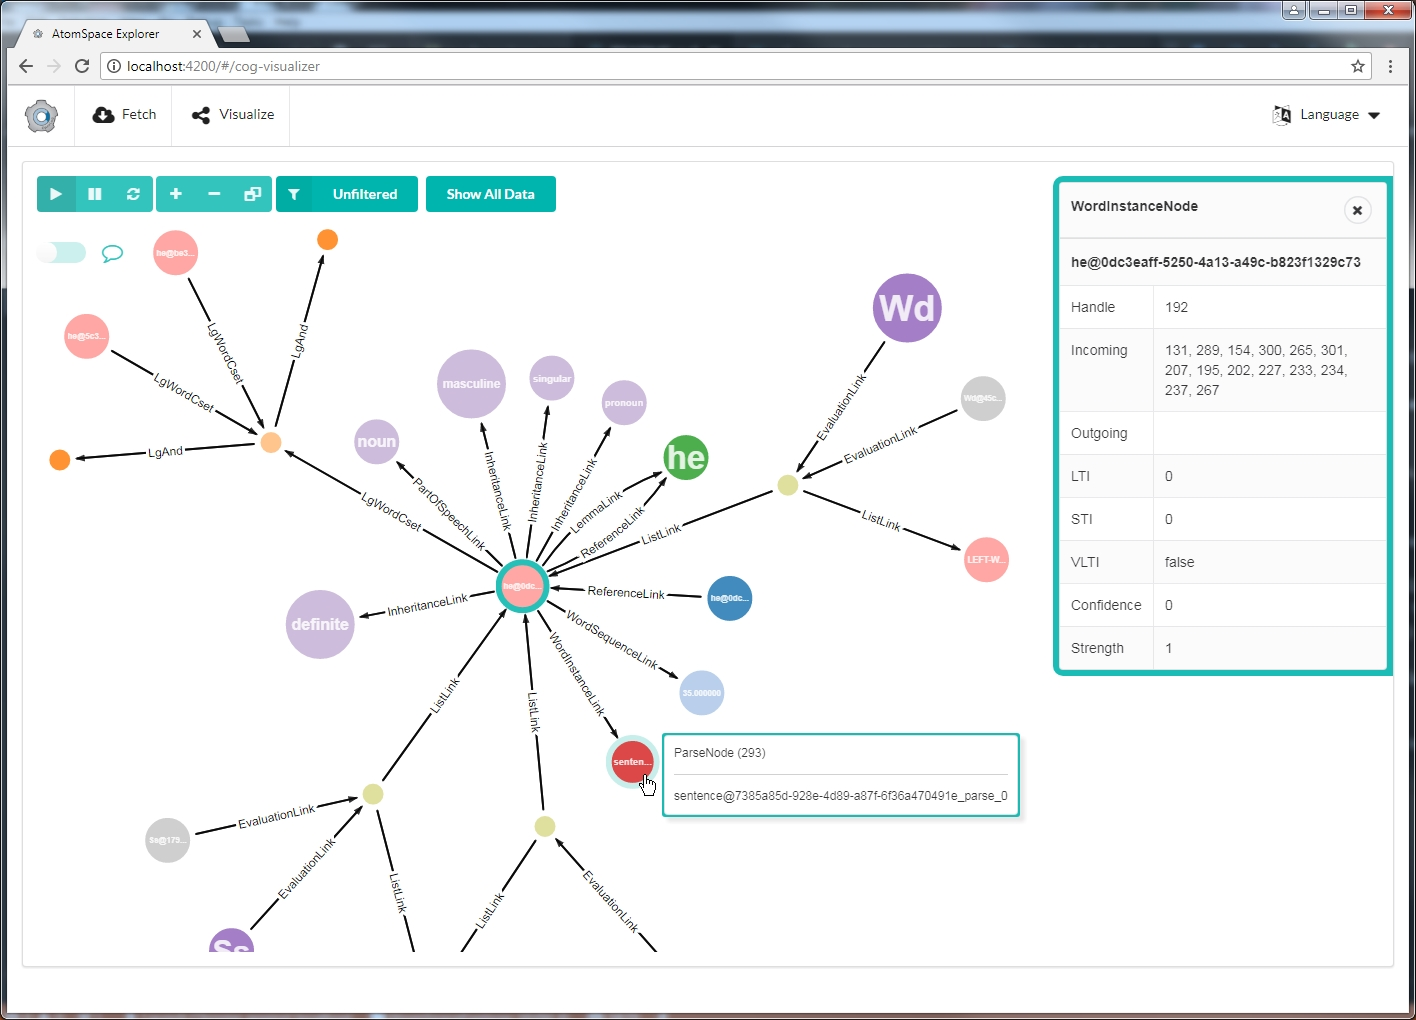
\includegraphics[width=1.0
\textwidth]{figures/Magistrale/atomspace_explorer}
\caption[AtomSpace Explorer ]{Atomspace example. By selecting an atom, you can get its unique ID, the type of atom (associated with an integer), incoming-set and outgoing-set, Strength and Confidence and much more.
\label{fig:atomspace_explorer}}
\end{figure}


\subsection{Atomese}\label{sec:atomese}

Because of these many and varied Atom types, constructing graphs to represent knowledge looks like a kind of \enquote{programming}. \\
The programming language is informally named \enquote{Atomese}. \\ 
Atomese is the concept of writing programs with Atoms. 
It vaguely resembles a strange mash-up of SQL, due to queriability, Prolog/Datalog, due to the logic and reasoning components, Lisp/Scheme, due to lambda expressions, Haskell/CaML, due to the type system, and rule engines, due to the graph rewriting and forward/backward chaining inference systems. \\

Atomese is not, and was never intended to be, a programming language with which humans would write source code, like Java, Python, LISP or Haskell. 
Rather, it is a language that computer algorithms, such as genetic programming systems, term rewriting systems and rule engines, would be able to manipulate. 
It is a graph database that pattern mining algorithms could search, manipulate and transform and is designed for easy self-introspection. \\

In its current form, Atomese was primarily designed to allow the generalized manipulation of large networks of probabilistic data by means of rules and inferences and reasoning systems. It extends the idea of probabilistic logic networks to a generalized system for algorithmically manipulating and managing data. The current, actual Atomese design has been heavily influenced by practical experience with natural-language processing, question answering, inferencing and the specific needs of robot control. \\

The use of the AtomSpace, and the operation and utility of Atomese, remains a topic of ongoing research (a re-evaluation of the OpenCog architecture is currently underway. A new OpenCog system called \enquote{Hyperon} is being studied \cite{goertzel_potapov_senna_singularitynet-opencog_team_2020}, introducing upgrades from Atomese to Atomese 2.0 \cite{DBLP:journals/corr/abs-2004-05267}, Distributed AtomSpace architecture \cite{distributed_2017, senna_2018, potapov_2020_1, potapov_2020_2} and much more) and design experimentation, as various AI and knowledge-processing subsystems are developed. These include machine learning, natural language processing, motion control and animation, deep-learning networks and vision processing, constraint solving and planning, pattern mining and data mining, question answering and common-sense systems, and emotional and behavioral psychological systems. Each of these impose sharply conflicting requirements on the AtomSpace architecture. The AtomSpace and Atomese are the current best-effort KR system for satisfying all these various needs in an integrated way.

\subsection{Pattern Engine, Unified Rule Engine and Relex2Logic}\label{sec:pattern_ur_engine}

Three more components of the OpenCog architecture are now introduced: Pattern Matcher, Unified Rule Engine and Relex2Logic. \\
Each of them is necessary for the following ones, in order of listing.
Unified Rule Engine is mostly built on top of the Pattern Matcher and it is applicable to rules written in a Scheme/Atomese representation, such as for Relex2Logic and PLN.

\subsubsection{Pattern Matcher}\label{sec:pattern_matcher}

OpenCog has a Pattern Matcher (PM), or Query Engine or Variable Unifier, that can be used to search the AtomSpace for specific patterns or arrangements or `templates' of atoms. 
The PM can be used from C++, Scheme or Python. \\
After specifying some (arbitrarily complex) arrangement of atoms, that is, a hypergraph consisting of Nodes and Links of several types, the PM can find all instances of that hypergraph in the AtomSpace. The pattern or template can have \enquote{holes} in it, locations that are variable, and so the pattern matcher can act to \enquote{fill in the blanks} when presented with a pattern that has blanks in it (better known by the expression: `grounding' a pattern). \\
For example, the VariableNode type are used to indicate these \enquote{blank spots}. \\
For a good introduction to these concepts, see \cite{baader_nipkow_1998}. Although, the PM implementation is considerably more sophisticated: it unifies multiple terms at once, automatically handles unordered terms (terms that can be in any order) and provides support for quotation, execution and evaluation. \\

For this project, patterns are specified using QueryLink type. \\
One creates the pattern-template that one wishes to search for. The pattern can be specified as a collection of trees, containing the VariableNodes, making up the graph. 
During the search, all matching graphs are found and the groundings are noted. \\
The QueryLink is used for graph-rewriting, thus these grounding are then pasted into a second pattern, to create a new graph. \\
In Section \ref{sec:domain_atomese}, practical applications will be presented to help understand these concepts as well.

\subsubsection{Unified Rule Engine}\label{sec:ure}

The Unified Rule Engine (URE) is a generic OpenCog rule engine operating on the AtomSpace and it can be used to implement any logic. \\
Two chaining modes are currently supported, Forward Chaining and Backward Chaining. \\
The strengths of the URE are:
\begin{itemize}
	\item Reads/writes knowledge directly from/to the AtomSpace
	\item It is generic, can be used to implement any logic, even higher order logics with some limitations
	\item Comes with a powerful control mechanism to speed up reasoning
\end{itemize}

It was used as a first approach to solve the problem faced in this project. It was later abandoned due to conceptual and practical problems in favour of a new approach (Section \ref{sec:search}), although, in the end, good ideas emerged that could solve these problems. See related Section [...sviluppi futuri]. \\
For these reasons, any other information related to URE is referred to \cite{geisweiller_2019} and the webpages linked to that.
%% TODO

\subsubsection{Relex2Logic}\label{sec:r2l}

This project handles a Natural Language Processing (NLP) module. Here, some components of OpenCog this module superficially uses, are very briefly presented. \\
The component on the top is called Relex2Logic (R2L). \\
R2L produces a certain form of predicate-argument structure for an English-language sentence. That structure roughly resembles classical propositional or predicate logic, thus the name. \\
It is pointless to go into the details of this module because, first of all, it became obsolete because its java rule engine and representation scheme were inadequate and knowledge extraction was too far removed from the reasoning and anaphora components; secondly, because the predicate-argument structure is produced by applying a set of rules to the RelEx format (see below), using the forward chainer provided by URE, which require a very good knowledge of the topic in order to be understood. \\

Thus, this module takes as input an English sentence and returns a relatively simple logical representation of it in Atomese. That is, a hypergraph composed of atoms that are associated with the words of the sentence and then structured to express the logic of it in the form of a hypergraph. The following example is used to better explain: \\
\begin{python}
	The English sentence: "The cat is an animal"

---------------- Result:
(EvaluationLink (stv 1 1)
  (PredicateNode 
    "is.v@5fdee4a0-7ad4-4aa7-9172-55a137c3dbdf" 
      (stv 9.75697e-13 0.00124844))
  (ListLink
    (ConceptNode 
      "cat.n@e425545c-ceea-4eee-931b-a6c312d66d58")
    (ConceptNode 
      "animal.n@1813a95c-0c44-46f6-bad3-7232f6ff8616")))

(InheritanceLink (stv 1 1)
  (ConceptNode 
    "cat.n@e425545c-ceea-4eee-931b-a6c312d66d58")
  (ConceptNode 
    "animal.n@1813a95c-0c44-46f6-bad3-7232f6ff8616"))

(EvaluationLink (stv 1 1)
  (PredicateNode 
    "is.v@5fdee4a0-7ad4-4aa7-9172-55a137c3dbdf" 
      (stv 9.75697e-13 0.00124844))
  (ListLink
    (ConceptNode 
      "cat.n@e425545c-ceea-4eee-931b-a6c312d66d58")))

(InheritanceLink (stv 1 1)
  (InterpretationNode 
    "sentence@c9bf0479-2636-4a8b-901c-38d1305ed29e_
parse_0_interpretation_$X" (stv 9.75697e-13 0.00124844))
  (DefinedLinguisticConceptNode 
    "DeclarativeSpeechAct" (stv 9.75697e-13 0.00124844)))

(ImplicationLink (stv 1 1)
  (PredicateNode 
    "is.v@5fdee4a0-7ad4-4aa7-9172-55a137c3dbdf" 
      (stv 9.75697e-13 0.00124844))
  (PredicateNode "be" (stv 9.75697e-13 0.00124844)))

(InheritanceLink (stv 1 1)
  (ConceptNode "animal.n@1813a95c-0c44-46f6-bad3-7232f6ff8616")
  (ConceptNode "animal"))

(InheritanceLink (stv 1 1)
  (ConceptNode "cat.n@e425545c-ceea-4eee-931b-a6c312d66d58")
  (ConceptNode "cat"))

(InheritanceLink (stv 1 1)
  (PredicateNode 
    "is.v@5fdee4a0-7ad4-4aa7-9172-55a137c3dbdf" 
      (stv 9.75697e-13 0.00124844))
  (DefinedLinguisticConceptNode 
    "present" (stv 9.75697e-13 0.00124844)))

(EvaluationLink (stv 1 1)
  (DefinedLinguisticPredicateNode 
    "definite" (stv 9.75697e-13 0.00124844))
  (ListLink
    (ConceptNode 
      "cat.n@e425545c-ceea-4eee-931b-a6c312d66d58")))
\end{python}

All the Atoms whose names contain the \textit{@} character are those that are associated with the words in the sentence. In this way, the same word in different places can take on different meanings and links. \\
However, these atoms (such as \textit{cat.n@...}, \textit{animal.n@...} and \textit{is.v@...}) are actually inherited by the concepts (ConceptNodes) that represent them, so `cat', `animal' and `is' (lines 35, 41, 45). \\ 
Moreover, the atom in line 4 perfectly describes the relationship between these three concepts in the sentence. \\

The processing pipeline for a sentence is: 
\begin{enumerate}
	\item Sentence $\Rightarrow$ Link-Grammar
	\item Link-Grammar $\Rightarrow$ RelEx
	\item RelEx $\Rightarrow$ Relex2Logic
\end{enumerate}

Step 1 performs a syntactic parse of a sentence, using the Link Grammar (LG) parser. \\

Step 2 converts the LG output into a dependency grammar (DG) format that is more closely aligned with de-facto DG standards. This includes the unpacking of some of the LG output into standard linguistic feature classifications, e.g. for person, number, tense, aspect, mood, voice. \\
This converter is called RelEx, a Narrow-AI component of OpenCog. It is an English-language semantic dependency relationship extractor, built on the Carnegie-Mellon Link Grammar parser. It uses a series of graph rewriting rules to identify subject, object, indirect object and many other syntactic dependency relationships between words in a sentence. That is, it generates the dependency trees of a dependency grammar. \\
Unlike other dependency parsers, RelEx attempts a greater degree of semantic normalization: for questions, comparatives, entities, and for modifying clauses, and sub-ordinate clauses. \\

Step 3 extracts the predicate-argument logical structure, as shown above.
